\section{Appendix: Evaluating Photo-$z$ Estimators}\label{sec:eval}

\textcolor{red}{This section could be entirely replaced with a citation to the comparative analysis work of Schmidt et al. (2019) when that paper is ready.}

This section provides more in-depth examples of how to comparatively evaluate different photo-$z$ estimators, in support of the proposed selection criteria put forth in \S~\ref{sec:sel}.


\subsection{Lessons from Surveys That Compare Photo-$z$ Estimators}\label{ssec:eval_lit}

\textbf{DESC photo-$z$ WG --} This science community is full engaged in the development of photo-$z$ routines and their optimization for LSST.
Their work is not reproduced here, \textcolor{red}{but we could add some citations.}

\textbf{Relevant photo-$z$ testing papers --} \cite{2010A&A...523A..31H} tested 18 different photo-$z$ codes on the same sets of simulated and real data and found no significantly outstanding method. 
\cite{2013ApJ...775...93D} test 11 different photo-$z$ codes on the CANDLES data set ($U$-band through infrared) and also find that no method stands out as the "best,'' and that there is a strong dependence of photo-$z$ accuracy on the SNR of the photometry (relevant for our tests at 1 year). 
They also found that most of the photo-$z$ codes underestimate their redshift errors.

\textbf{Lessons from DES --} \cite{2014MNRAS.445.1482S} use the science verification data (200 square degrees of $grizY$ photometry to a depth of $i_{AB}=24$ magnitudes) of the Dark Energy Survey (DES) to evaluate several photometric redshift estimators. 
They found that the Trees for Photo-$z$ code (TPZ; \citealt{2013ascl.soft04011C}) provided the most accurate results with the highest redshift resolution, and that template-fitting methods also performed well -- especially with priors -- but that in general there was no clear "winner.''

\textbf{Lessons from SDSS --} \cite{2016MNRAS.460.1371B} describes the photo-$z$ adopted for the SDSS DR12. They first use an empirical technique with a large training set to estimate the redshift and it's error, and then fit SED templates with that redshift in order to obtain additional galaxy information such as $K$-correction and spectral type. (Note: \textit{They call it a hybrid technique, but the photo-$z$ sounds like it comes solely from the local linear regression, basically an interpolation in the color-redshift relation}.)

\textbf{Lessons from the HSC Strategic Program --} \cite{2018PASJ...70S...9T} provides a comparative analysis of several photo-$z$ algorithms applied to their data set, and the program's website\footnote{\url{https://hsc-release.mtk.nao.ac.jp/doc/index.php/photometric-redshifts/}} provides comparative analysis plots for each of them.

\textbf{Lessons from Lucy's work --} Summer student Lucy Halperin (UW 2016, with Melissa Graham) took what we call the "Brown'' catalog\footnote{We call it the Brown catalog because it uses the SEDs from \cite{2014ApJS..212...18B}} made by Sam Schmidt, with simulated 10-year LSST-like magnitude uncertainties, and ran it through 2 machine learning (ANNz and TPZ) and 2 template-fitting (LePhare and BPZ) photo-$z$ codes. All four returned sets of photo-$z$ with similar standard deviations and biases, but the template-fitting codes were more prone to failures and outliers. Lucy's work found that for template-fitting photo-$z$ codes, the choice of template SED set does make a significant difference in the results, particularly regarding photo-$z$ outliers -- however, this may have been particular to the use of the "Brown''-based galaxy catalog.


\subsection{A Preliminary Application of Algorithms to LSST-like Photometry}\label{ssec:eval_ex}

We apply a couple of of-the-shelf estimators to simulated LSST photometry to demonstrate a few statistical techniques for comparing photometric redshifts.
We have used simulated galaxy catalogs (\S~\ref{sssec:eval_ex_cats}) and three different photo-$z$ estimators (\S~\ref{sssec:eval_ex_estimators}) to generate photometric redshifts. 
We then apply a series of diagnostics to evaluate and compare their performance (\S~\ref{sssec:eval_ex_comp}).
Since this is mainly for {\it demonstrative} purposes, the estimators themselves have not been optimized to return the most accurate photo-$z$, and some minor mistakes have been left uncorrected.

\subsubsection{Simulated Catalogs}\label{sssec:eval_ex_cats}

We use a randomly chosen 30000 galaxy test subset of the \textsc{LC\_DEEP\_Gonzalez2014a} catalog, which is based on the Millennium simulation \citep{2005Natur.435..629S} and the galaxy formation models of \cite{2014MNRAS.439..264G} and constructed using the lightcone techniques described by \cite{2013MNRAS.429..556M}. We impose a limit on the true catalog redshift of $z<3.5$, and a limit on the apparent $i$-band magnitude of $i<25.5$, and furthermore require galaxies to be detected in the three filters $gri$. The latter requirement means that the test galaxies' apparent magnitude is brighter than a limit defined by a signal-to-noise ratio $<5$ in all three filters $gri$. This limit depends on the number of years of survey elapsed, and since we want to use the same set of test galaxies to analyze the algorithms' results early in the survey, we require this $gri$ non-detection with the expected limits after only 1 year of LSST. These restrictions mean that we end up with a catalog that has with fewer faint galaxies than will be in the LSST 10-year catalogs, and so the 10-year results we consider here are optimistic (but that's fine for our purposes). These restrictions are imposed prior to the random selection of 30000 test galaxies from the larger catalog. We then simulate 4 versions of the test galaxy catalog with errors appropriate for $1$, $2$, $5$, and $10$ years of LSST. We calculate galaxy magnitude uncertainties that are appropriate for the elapsed survey time, and observed photometry is simulated by adding a random scatter proportional to the uncertainties.

In addition to the test set, we need a training set of galaxies for the machine-learning algorithm to serve as a spectroscopic redshift catalog. Spectroscopic data sets containing tens of thousands of galaxies down to $i>25$ and out to $z>3$ are certainly possible, e.g., the VIMOS Ultra Deep Survey (VUDS; \citealt{2015A&A...576A..79L}). Assuming that the LSST will cover a spectroscopic field like the VUDS to the full 10-year depth during commissioning or with a first-year deep drilling field, we use as our training set a sample of 30000 catalog galaxies with photometric uncertainties equivalent to a 10-year LSST. This training set has the same redshift and magnitude distribution and limits as the galaxy catalogs, which may not be the case for a real spectroscopic set.

\subsubsection{Considered Photo-$z$ Estimators}\label{sssec:eval_ex_estimators}

Here we've considered one template-fitting and one machine-learning photo-$z$ algorithm. Hybrid photo-z estimators attempt to mitigate the flaws of either process (e.g., the SDSS DR12 photo-$z$ estimator by \citet{2016MNRAS.460.1371B}, or the Gaussian Processes estimator described by \citet{2017ApJ...838....5L}).

\textbf{Bayesian Photometric Redshifts} (BPZ; \citealt{2000ApJ...536..571B}) is a template-fitting algorithm with a magnitude prior\footnote{\url{http://www.stsci.edu/~dcoe/BPZ/}}. We use all default parameters, including the $i$-band for the magnitude prior, except that we supply the CFHTLS set of SED templates. This set is 66 SEDs that were used for the CFHTLS photo-$z$ paper and are from \cite{2006A&A...457..841I}, and they were interpolated from the CWW and Kinney models.

%Note: run with 100 trees was 1h 47m.
\textbf{Trees for Photometric Redshifts} (TPZ; \citealt{2013ascl.soft04011C,2013MNRAS.432.1483C}) is a machine learning algorithm that uses prediction trees and a training set of galaxies with known redshifts. We use all the default parameters from the example, except we increase the number of trees from 4 to 10 (this was set low in the provided example to decrease run time). Since the number of realizations is 2, this is a total of 20 trees. As shown in \cite{2013MNRAS.432.1483C}, the bias and scatter of the resulting photo-$z$ improve the most as the number of trees is increased to 20, and continues to improve more mildly to 100, and then are not much improved beyond 100 trees (i.e., their Figure 9). We also set the maximum redshift to 3.5 and the number of redshift bins to 350. We include both magnitudes and colors and their uncertainties as attributes to be used in the prediction trees, as Lucy's work found that this led to better results. From the TPZ output files, we take as $z_\mathrm{phot}$ the mode of the redshift distribution instead of the mean because this is the peak of the distribution (most likely redshift). \textit{Note: I may have misunderstood how TPZ uses the photometric uncertainties. I thought it treated errors differently from other \texttt{Attributes}, but perhaps it uses them just the same. That makes sense, but means it is inappropriate to include photometric errors as {ttc Attributes} if the train and test sets have different photometric precision.} In case a training set with LSST photometric uncertainties at the level of a 10-year survey is not available from commissioning or a dedicated deep drilling survey by the end of year 1, we also simulate the photo-$z$ results with a training set that has the same level of photometric uncertainty as the test set.

\textbf{Color-Matched Nearest-Neighbors} (CMNN; Graham et al. 2018) is a photo-$z$ estimator that uses the Mahalanobis distance in color-space to match a galaxy to a training set. We simulate photo-$z$ at 1, 2, 5, and 10 years using a test set of 20000 and a training set of 60000. Training set has the same photometric depth as the test set.


\subsubsection{Analysis and Results}\label{sssec:eval_ex_comp}

In this section we demonstrate several analysis techniques for comparing the output of different photo-$z$ estimators, discussing each in turn below.

\smallskip \noindent \textbf{The $z_\mathrm{true}$--$z_\mathrm{phot}$ Diagram} \\
Figure \ref{fig:tzpz} shows the photo-$z$ results in $z_\mathrm{true}$--$z_\mathrm{phot}$ diagrams, which are a typical way to visually asses the output. Galaxies are plotted with a semi-transparent black dot so that density and clustering of points is clear, and galaxies that end up designated as "outliers'' are over-plotted with a more opaque red dot. Problems such as outlier structure from e.g., color-$z$ degeneracies, and quantization of $z_\mathrm{phot}$ is obvious in these kinds of diagrams, as well as a decent overall impression of the scatter and bias. Even though our runs with these estimators have not been optimized, we can make an "example'' assessment of these figures to compare the two estimators.
\textbf{BPZ:} Overall the results are quite poor even with the LSST 10-year predicted photometry, especially the amount of quantization at $z_\mathrm{phot}>1.5$. We find that the results are not improved if we remove the magnitude prior, or use a different SED template set such as those from \cite{2014ApJS..212...18B}. We do know from Lucy's work that the choice of SED template set has a significant impact on the results (this is actually widely known) -- in Lucy's work, the best results were achieved when we used the Brown SEDs with a galaxy catalog for which the photometry was simulated using those same SEDs. However, it's less straightforward to identify the "best'' template SEDs to use with the Euclid galaxy catalog (or real data for that matter). \cite{2014MNRAS.439..264G} describes the wide variety of stellar population spectral synthesis models they used, but it would take quite some work to get them all together into a single catalog to provide to BPZ.
\textbf{TPZ:} The results are quite poor 1 and 2 years, with a lot of quantization in the photo-$z$ and many outliers at low and high redshift, but are significantly improved at 10 years. It is very interesting that there is actually a large improvement if the training set does not have better photometric errors than the test set (i.e., compare the 1 and 2 year results in the third row to the second row), but this may just be related to how we've included the errors as \texttt{Attributes}. Either way, TPZ is sensitive to the provided training set, so an extended investigation into what would truly be a realistic 1 year spectroscopic training set for LSST should be done (e.g., different redshift distributions, different magnitude limits). Although TPZ appears to give better accuracy, we also need to ensure that it gives realistic precision for it's photo-$z$ results.

\smallskip \noindent \textbf{Statistical Measures} \\
The important statistical measures that are typically used to assess photo-$z$ results are based on the photo-$z$ error, $\Delta z_{(1+z)} = (z_\mathrm{spec}-z_\mathrm{phot})/(1+z_\mathrm{phot}$. We measure the robust standard deviation in $\Delta z_{(1+z)}$, $\sigma_{\Delta z_{(1+z)}}$ (i.e., "robust'' because it is the standard deviation of galaxies within the IQR); the robust bias, which is the mean deviation $\overline{\Delta z}_{(1+z)}$; and the fraction of outliers, $f_\mathrm{out}$, which is the fraction of galaxies with $|\Delta z_{(1+z)}|> 0.06$ and $>3\sigma_\mathrm{IQR}$ (i.e., must be greater than whichever constraint is larger). In the community sometimes the median deviation in $\Delta z_{(1+z)}$ over all galaxies is used instead of the mean deviation of galaxies within the IQR, but we find the two are comparable. In Figure \ref{fig:stats} we demonstrate a convenient way to statistically compare the results from multiple photo-$z$ estimators. In this case we are comparing the values of these statistical measures when the photo-$z$ estimators are run on galaxy catalogs simulated to represent the 1, 2, 5, and 10 year DRP from LSST (colored lines), for both BPZ (left) and TPZ (right). Different estimators for the same year could also be plotted in a single graph. From these statistical measures it is obvious, for example, that the photo-$z$ from TPZ outperform those from BPZ at all years. In Figure \ref{fig:stat_stat} we show examples of how to compare the statistical measures for the full catalog (i.e., $0.3 \leq z_\mathrm{phot} \leq 3.0$) for different photo-$z$ estimators by plotting, e.g., the fractions of failures versus the outliers, or the bias versus the standard deviation.

\smallskip \noindent \textbf{Photo-$z$ Uncertainties, $\delta z_\mathrm{phot}$} \\
In Figure \ref{fig:pzpze} we demonstrate a way to assess the photo-$z$ uncertainties, $\delta z_\mathrm{phot}$, that come out of the estimators: we plot $z_\mathrm{phot}$--$\delta z_\mathrm{phot}$ in the main axis, and above and to the side plot the distributions in $\delta z_\mathrm{phot}$, $z_\mathrm{phot}$, and for comparison, $z_\mathrm{true}$. With BPZ, we can see a strict floor in the photo-$z$ uncertainty that increases with redshift (i.e., the uncertainties are bogus, though this could be a fault of mine in running the code and not of the code itself). For both BPZ and TPZ we can see that in some cases the clumps causing a quantization in photo-$z$ also have high photo-$z$ uncertainty, suggesting that a simple cut on $\delta z_\mathrm{phot}$ could return a sample for which the photo-$z$ distribution matches the true distribution. However, there are other clumps in photo-$z$ that have a relatively low uncertainty. Overall, from these plots we could conclude that the TPZ algorithm returns a redshift distribution that is more similar to the true distribution. Another option here is to plot the photo-$z$ error ($\Delta z_{(1+z)}$).

\smallskip \noindent \textbf{The Posterior Probability Density Function, $P(z)$} \\
In Figure \ref{fig:zpdf} we plot examples of the posterior probability density functions output by the BPZ and TPZ algorithms for two test galaxies. One galaxy was chosen as a random representative of galaxies for which an inaccurate and imprecise photo-$z$ was returned from both BPZ and TPZ for all years (top panel of Figure \ref{fig:zpdf}). The other was chosen as a random representative of galaxies which experienced a large and consistent improvement in both the accuracy and precision of its photo-$z$ from year 1 to 10, for both BPZ and TPZ (bottom panel of Figure \ref{fig:zpdf}). These kind of plots demonstrate, for example, the quantization in the TPZ photo-$z$ in the PDFs (this may be related to a mistake in the TPZ input).

\smallskip \noindent \textbf{Q-Q Plots} \\
In Figure \ref{fig:qq} we show an example of a quantile-quantile plot using the true $vs.$ the photometric redshift. Each point represents the $z_\mathrm{true}$ and $z_\mathrm{phot}$ for a given quantile, and since the two distributions we are comparing have the same total number of objects (we've neglected any galaxies that have failed to return a photo-$z$), we're simply using $1/N$ as the quantiles. If the Q-Q plot is linear with a slope of 1, we would know the distributions of $z_\mathrm{phot}$ would match that of $z_\mathrm{true}$. In Figure \ref{fig:qq} we can see for both BPZ and TPZ that this is not the case, but that BPZ is worse.

\clearpage

\begin{figure*}
\begin{center}
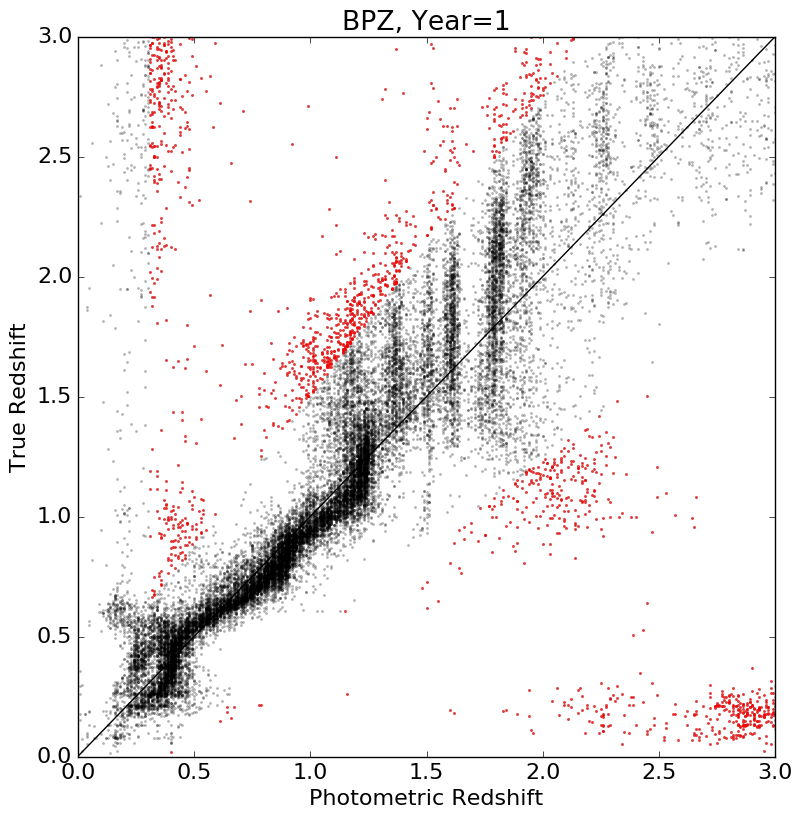
\includegraphics[width=4.0cm]{figures/BPZ_Euclid_Y1_tzpz.png}
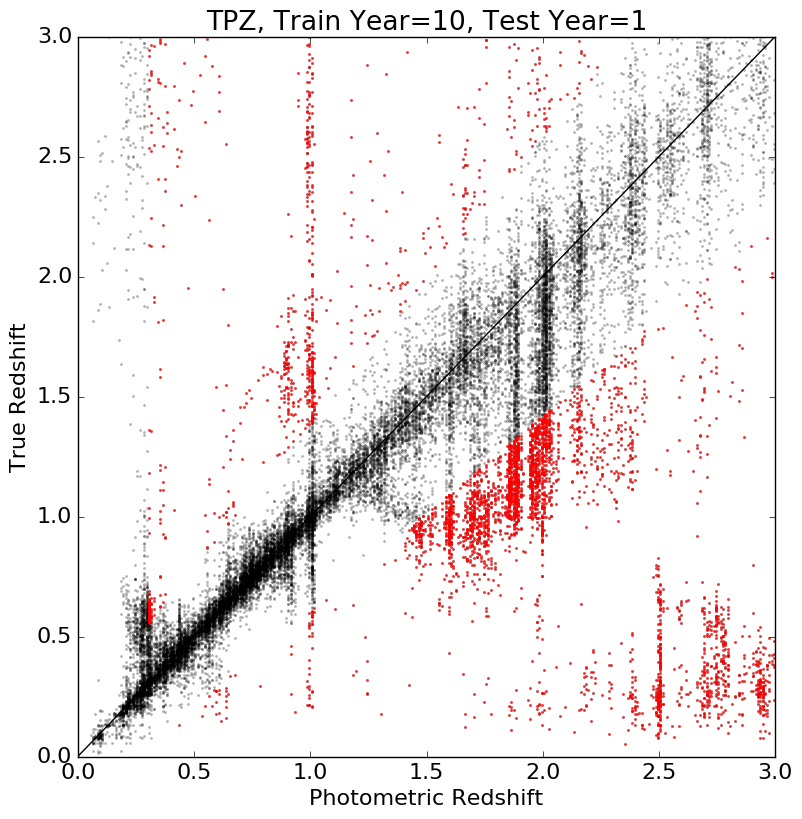
\includegraphics[width=4.0cm]{figures/TPZ_Euclid_10Y1_tzpz.png}
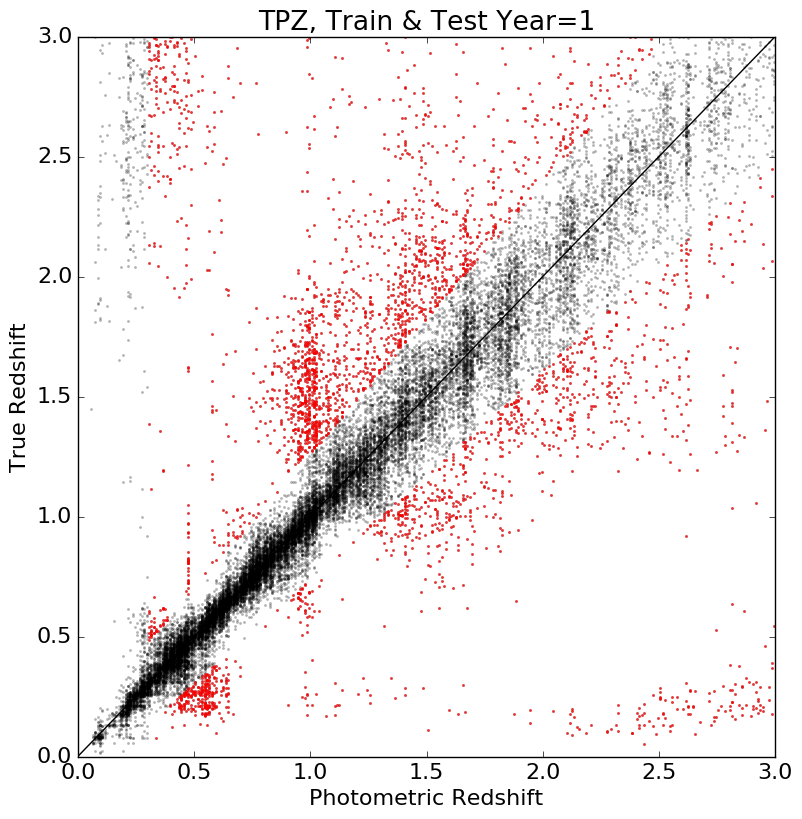
\includegraphics[width=4.0cm]{figures/TPZ_Euclid_1Y1_tzpz.png}
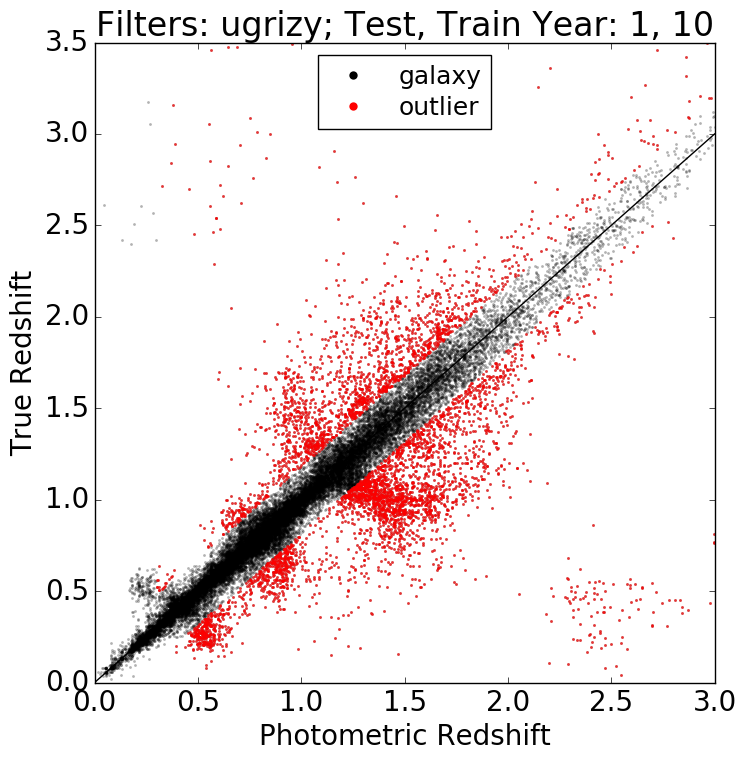
\includegraphics[width=4.0cm]{figures/CM_10Y1_tzpz.png}
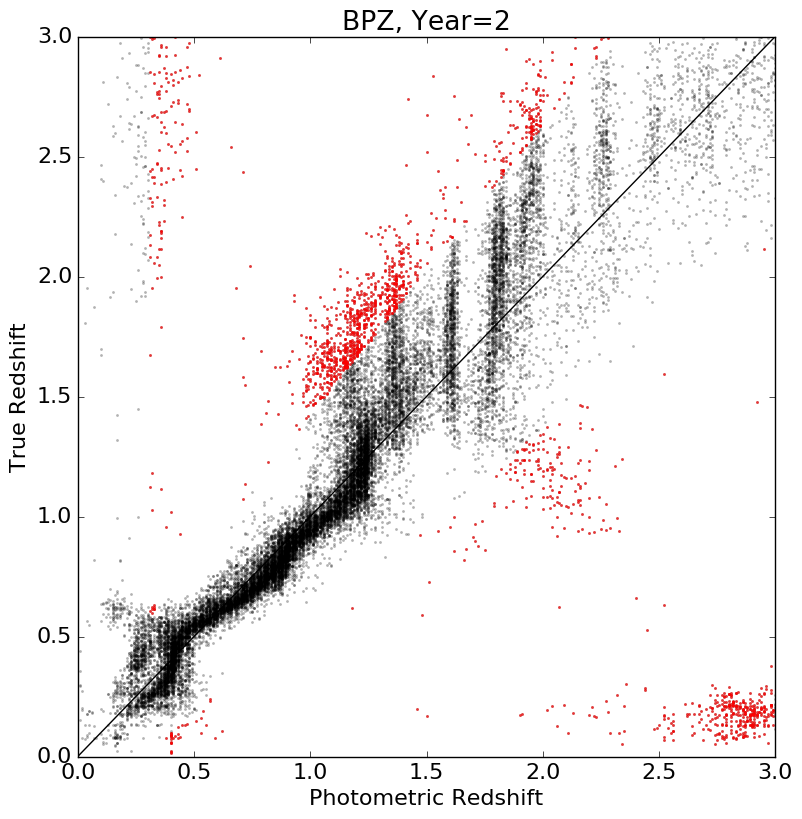
\includegraphics[width=4.0cm]{figures/BPZ_Euclid_Y2_tzpz.png}
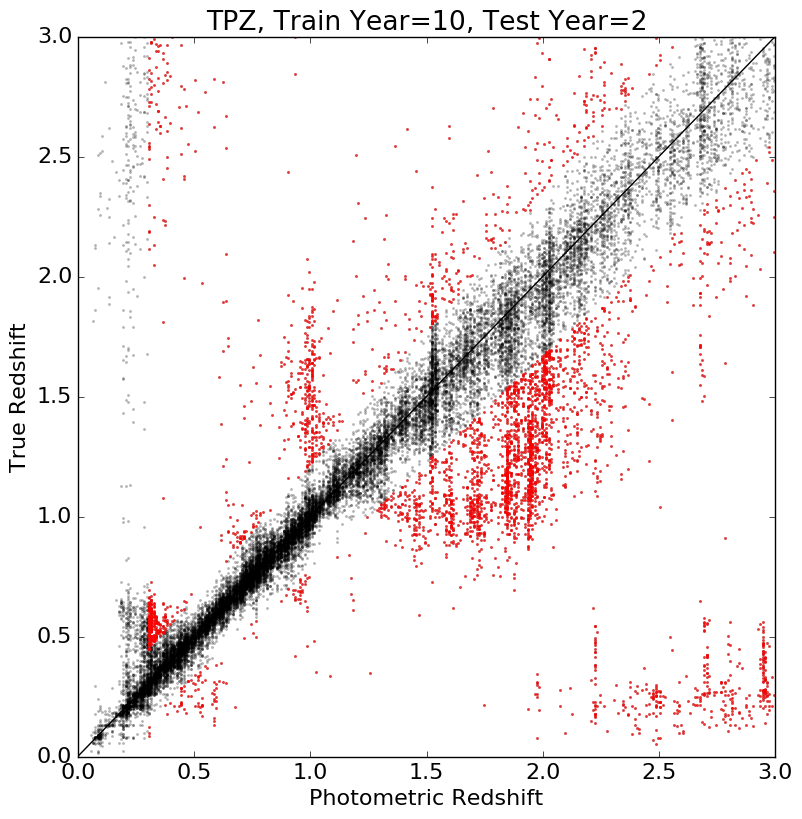
\includegraphics[width=4.0cm]{figures/TPZ_Euclid_10Y2_tzpz.png}
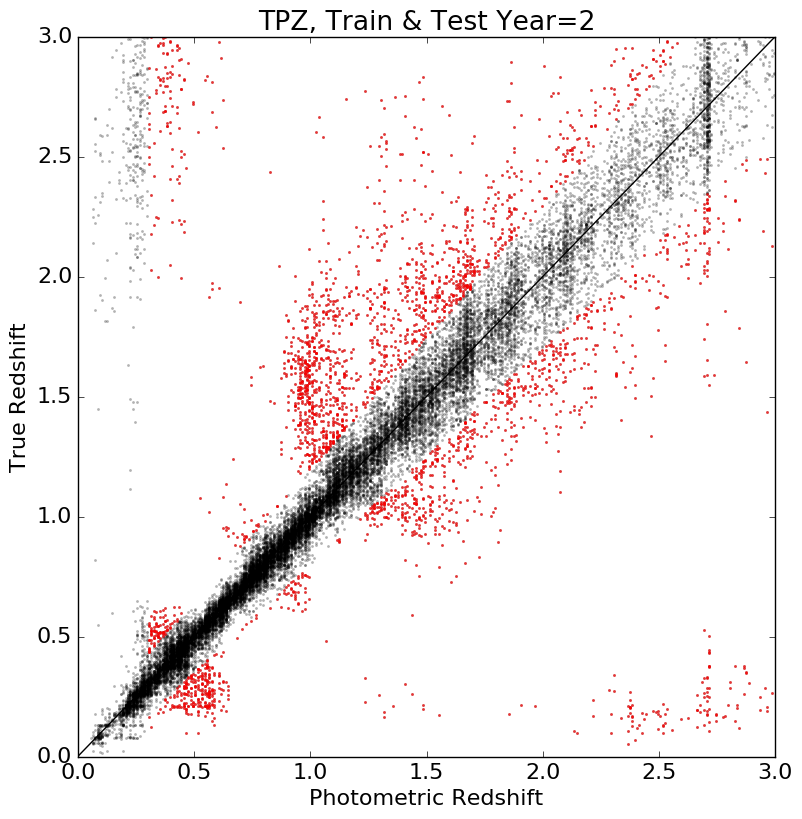
\includegraphics[width=4.0cm]{figures/TPZ_Euclid_2Y2_tzpz.png}
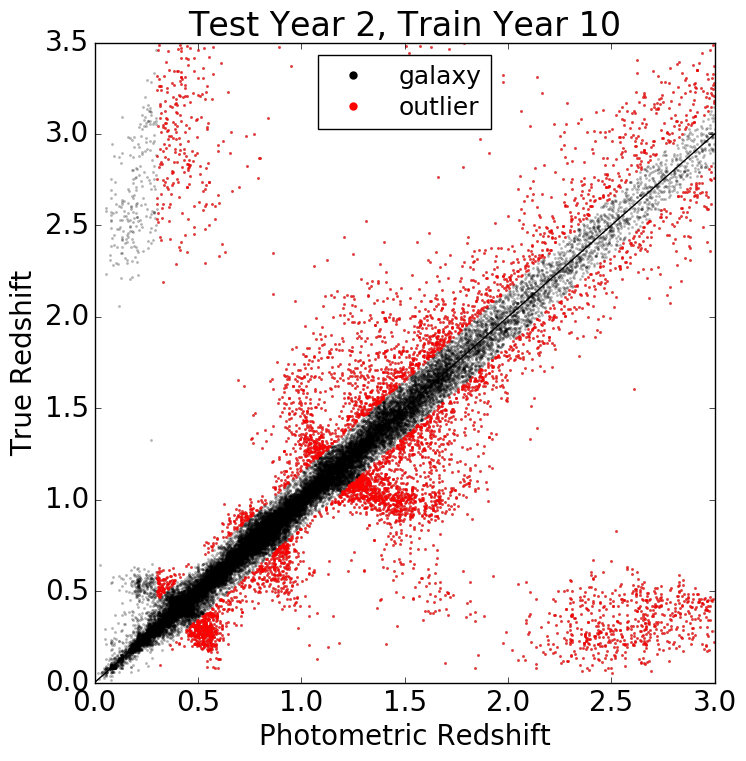
\includegraphics[width=4.0cm]{figures/CM_10Y2_tzpz.png}
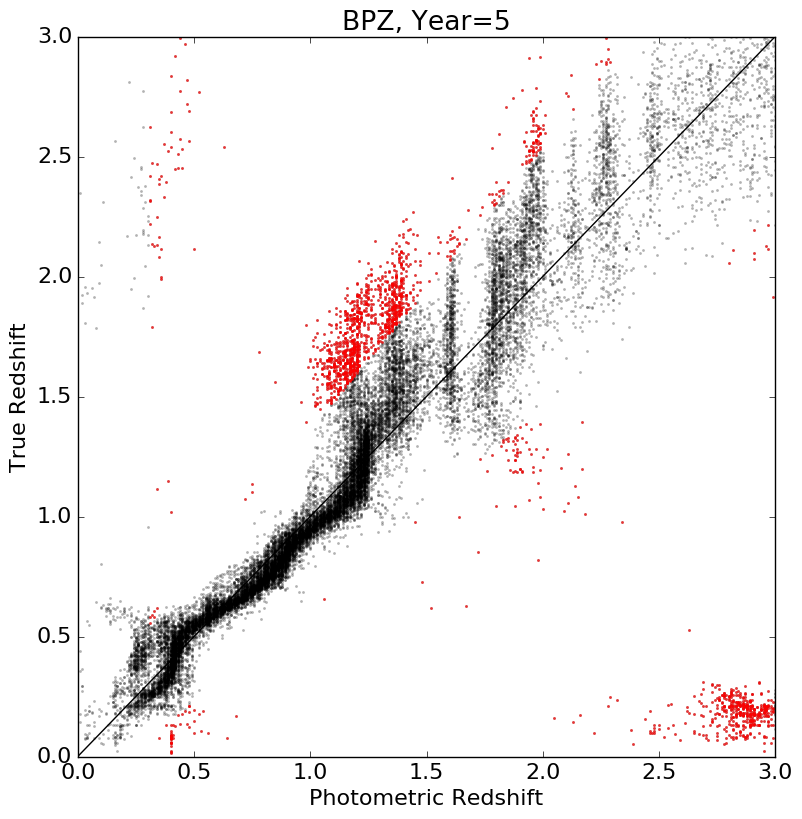
\includegraphics[width=4.0cm]{figures/BPZ_Euclid_Y5_tzpz.png}
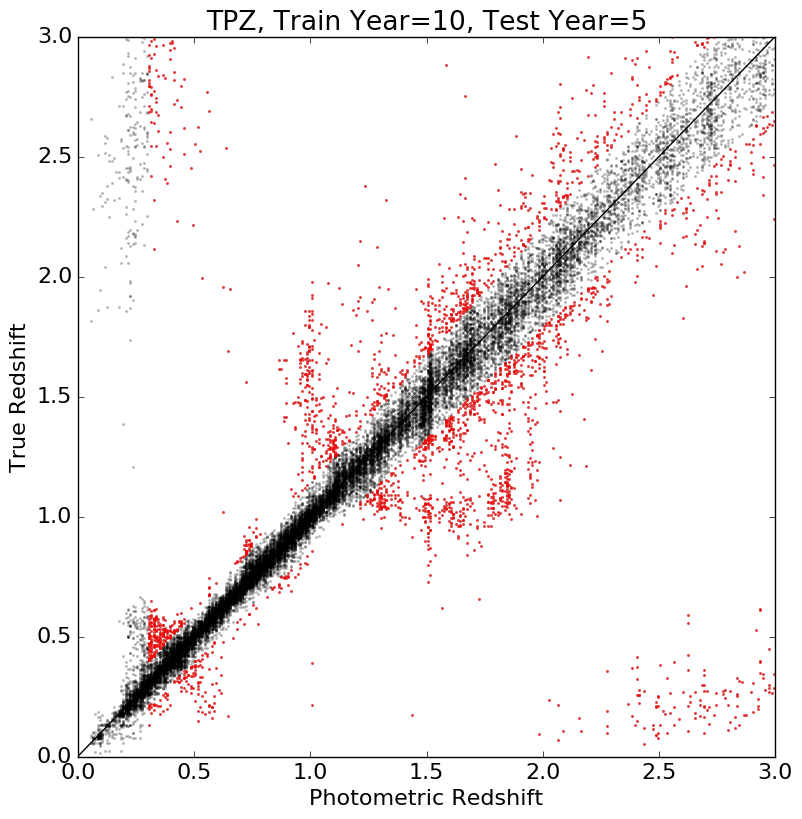
\includegraphics[width=4.0cm]{figures/TPZ_Euclid_10Y5_tzpz.png}
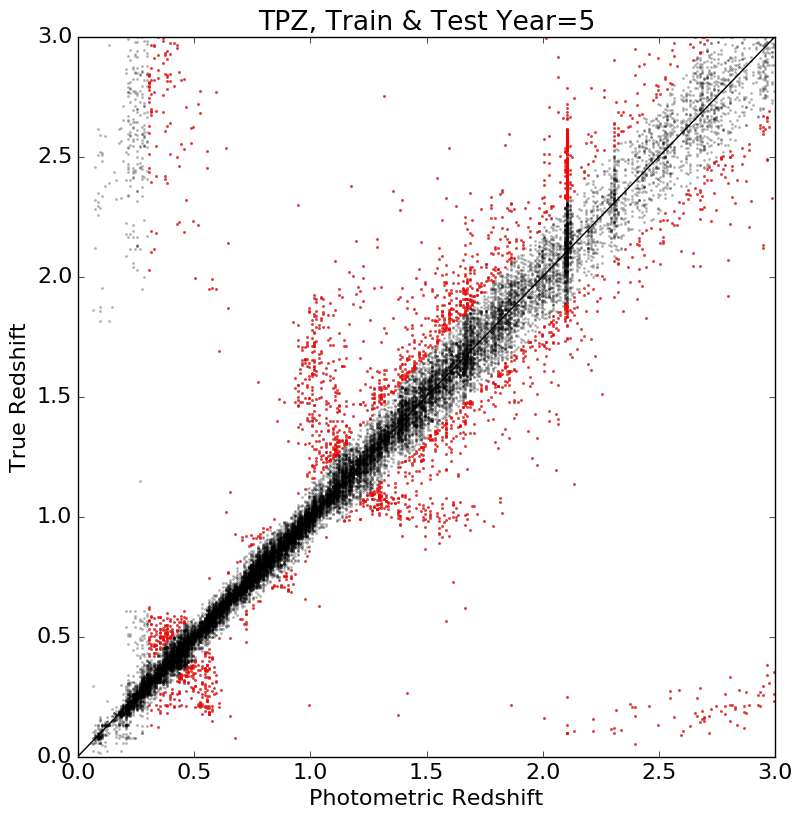
\includegraphics[width=4.0cm]{figures/TPZ_Euclid_5Y5_tzpz.png}
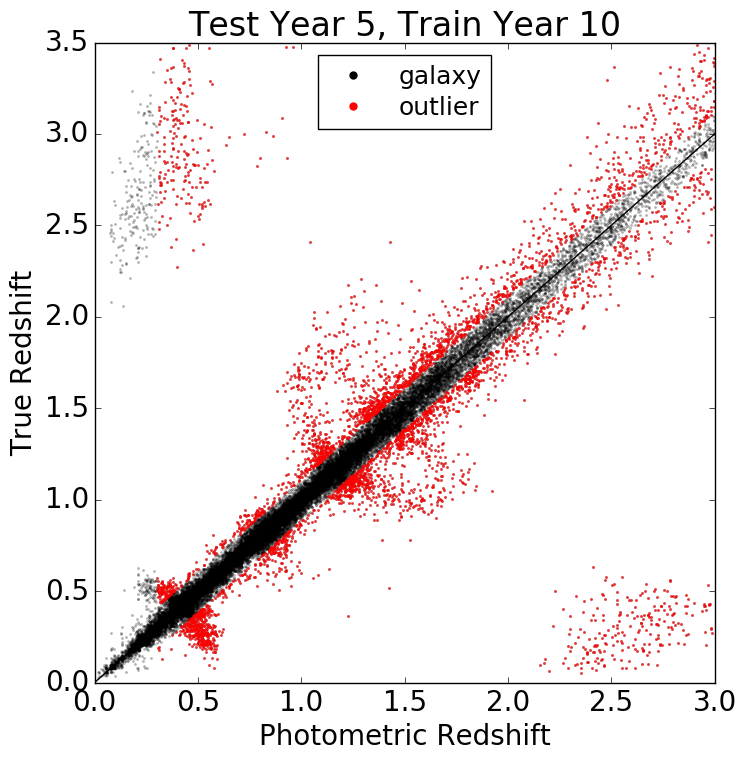
\includegraphics[width=4.0cm]{figures/CM_10Y5_tzpz.png}
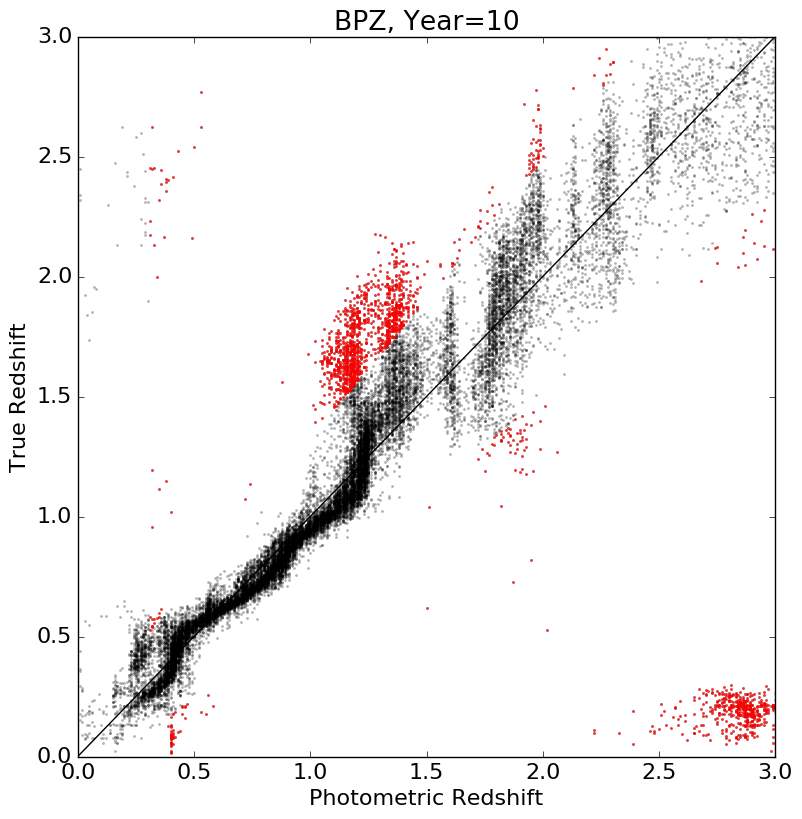
\includegraphics[width=4.0cm]{figures/BPZ_Euclid_Y10_tzpz.png}
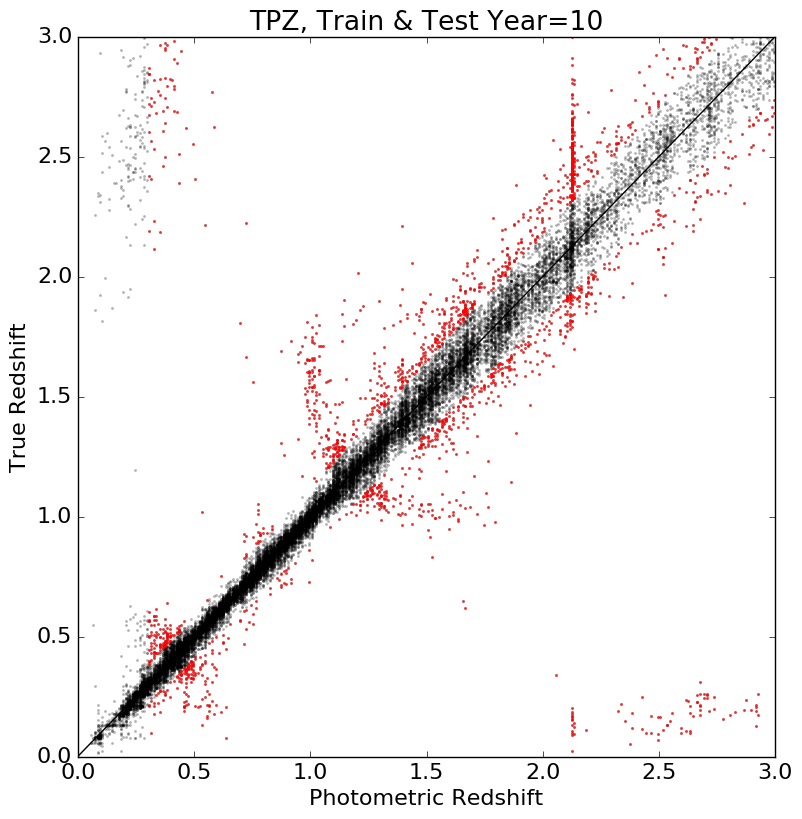
\includegraphics[width=4.0cm]{figures/TPZ_Euclid_10Y10_tzpz.png}
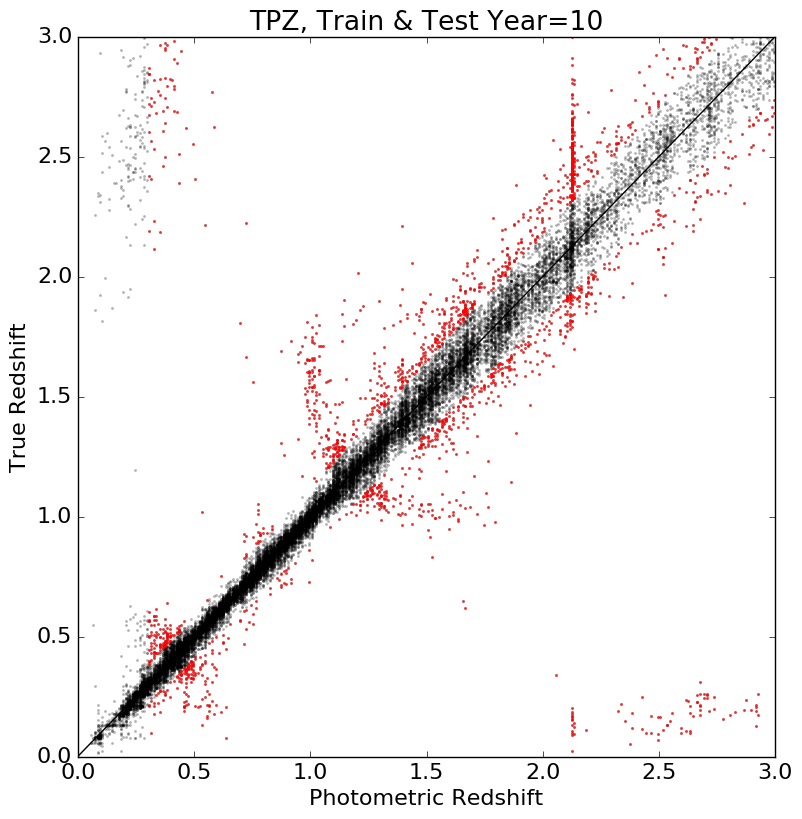
\includegraphics[width=4.0cm]{figures/TPZ_Euclid_10Y10_tzpz.png}
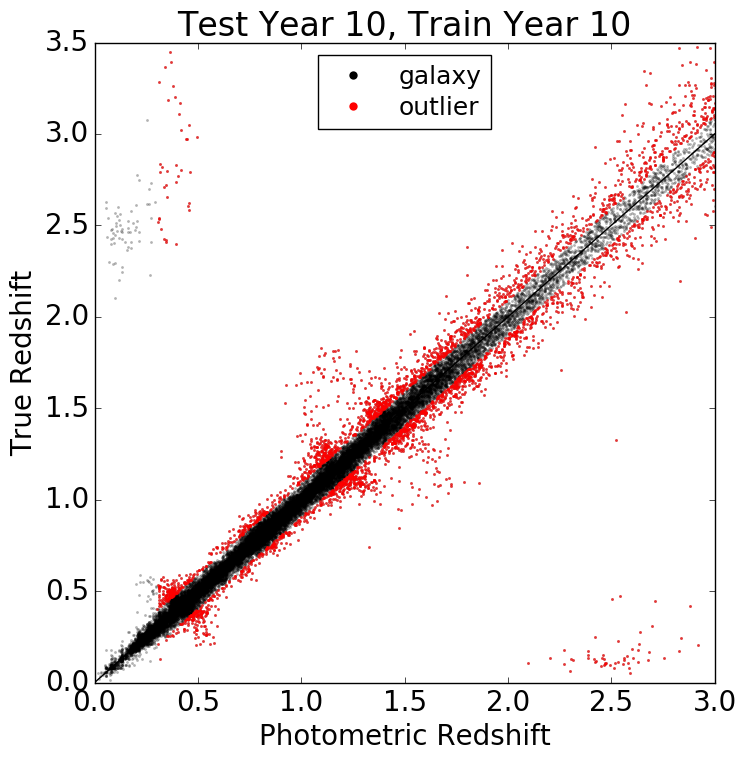
\includegraphics[width=4.0cm]{figures/CM_10Y10_tzpz.png}
\caption{Examples of $z_\mathrm{true}$--$z_\mathrm{phot}$ plots for a variety of algorithms (by column), for 1, 2, 5, or 10 years of survey time elapsed (top to bottom). Galaxies that are statistical outliers are shown in red. \textbf{Left:} results for the BPZ algorithm. \textbf{Center-left:} results for the TPZ algorithm with a 10-year training set. \textbf{Center-right:} results for the TPZ algorithm with a co-evolving training set. \textbf{Right:} results for nearest-neighbors color-matching algorithm, with 50000 test galaxies and $10^6$ training set galaxies with co-evolving photometric errors. \label{fig:tzpz}}
\end{center}
\end{figure*}

\begin{figure*}
\begin{center}
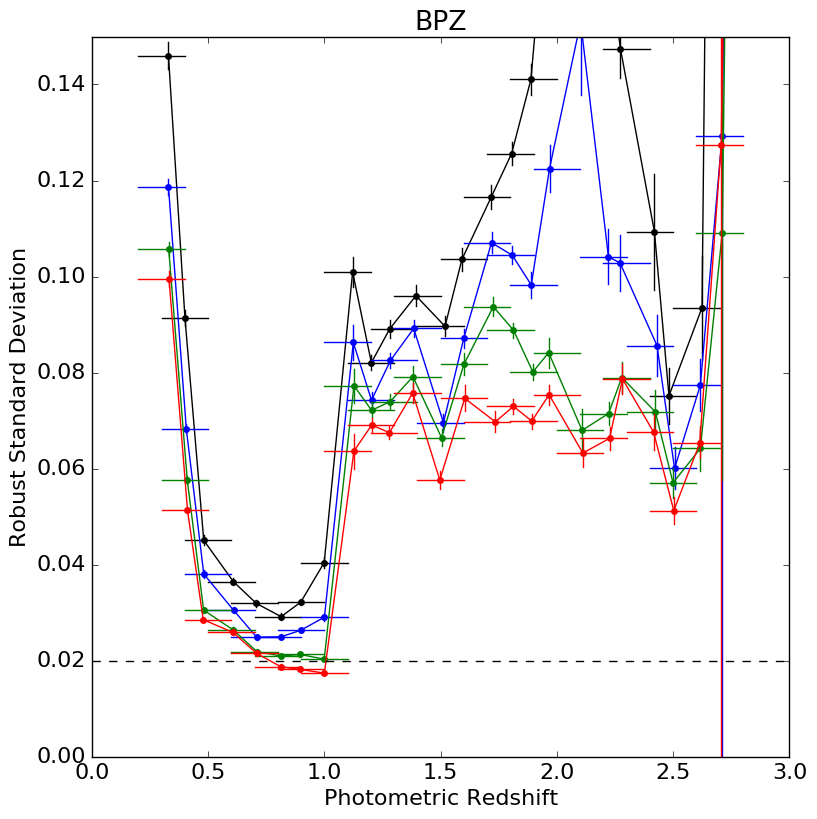
\includegraphics[width=6cm]{figures/BPZ_Euclid_IQRs.png}
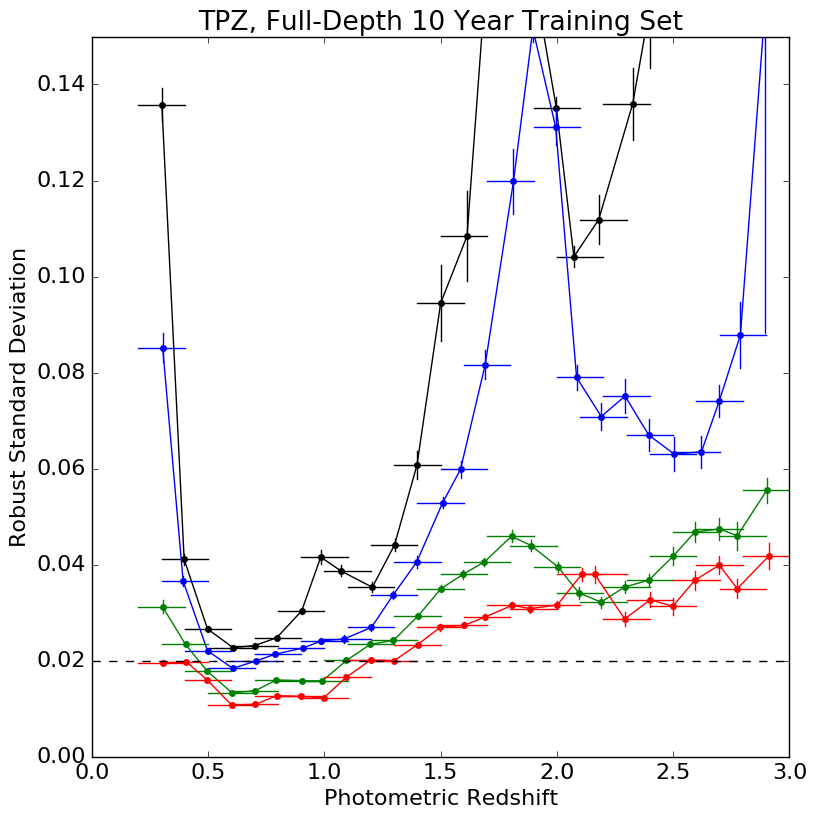
\includegraphics[width=6cm]{figures/TPZ_Euclid_TFD_IQRs.png}
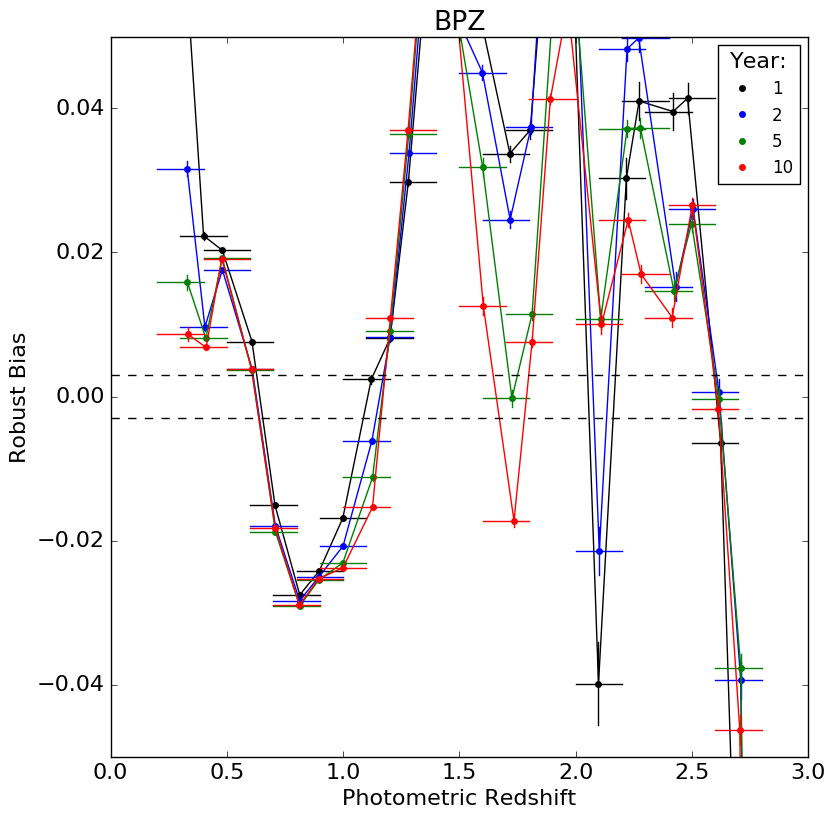
\includegraphics[width=6cm]{figures/BPZ_Euclid_bias.png}
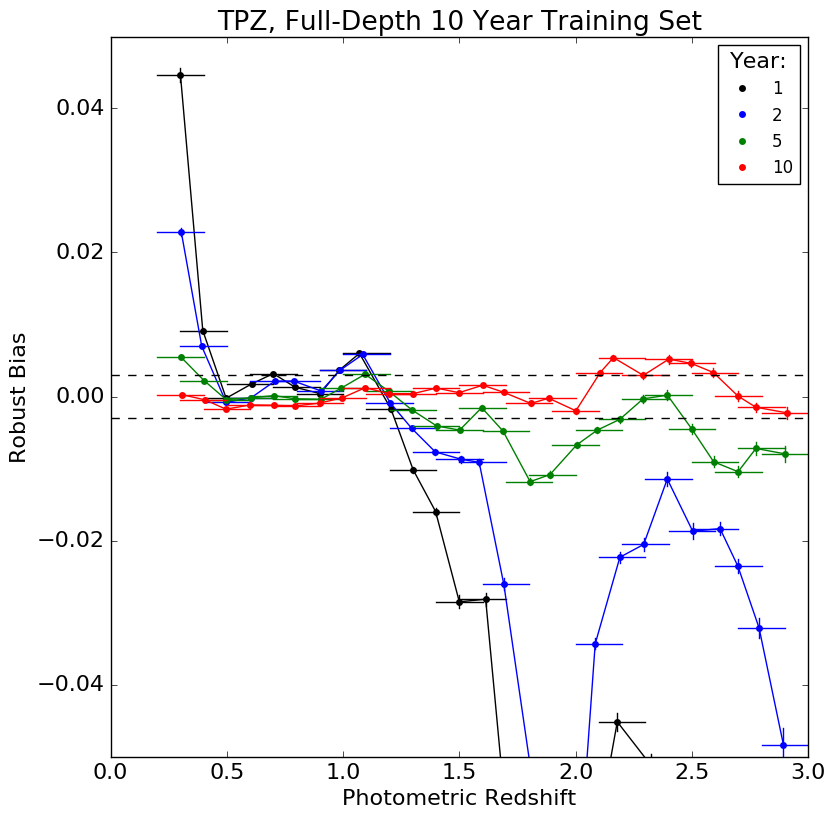
\includegraphics[width=6cm]{figures/TPZ_Euclid_TFD_bias.png}
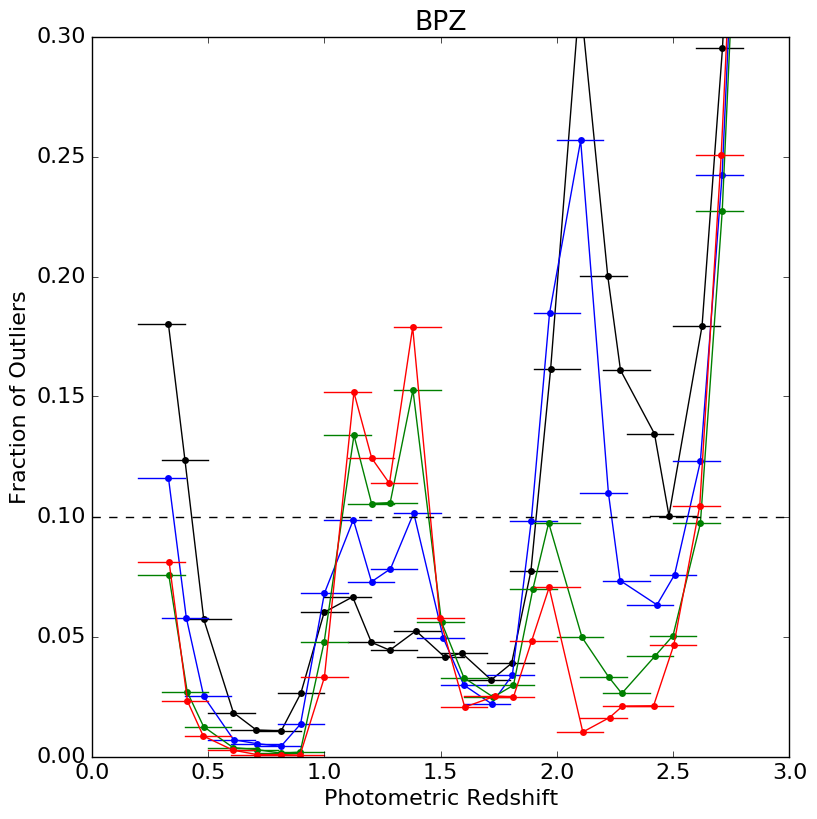
\includegraphics[width=6cm]{figures/BPZ_Euclid_fout.png}
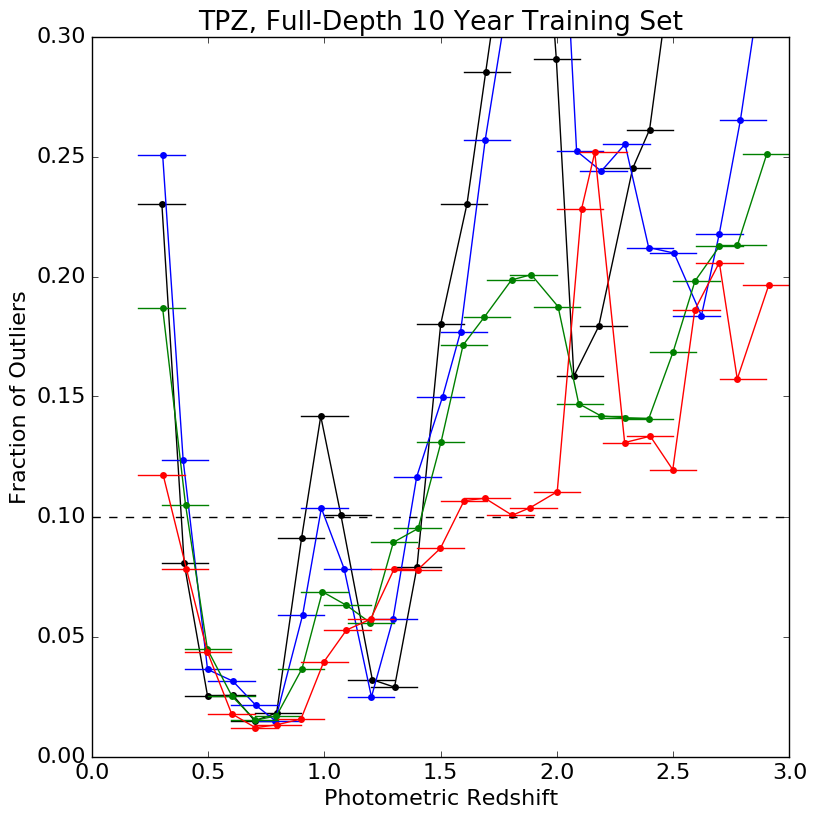
\includegraphics[width=6cm]{figures/TPZ_Euclid_TFD_fout.png}
\caption{Examples of a statistical measures of the photo-$z$ results from BPZ (left) and TPZ with an evolving training set (right) for simulated catalogs at 1 to 10 years (line colors as in plot legends). From top to bottom we show the robust standard deviation from the IQR, the robust bias, and the fraction of outliers as a function of photo-$z$, with matched $x$- and $y$-axes to facilitate comparison between BPZ and TPZ. \label{fig:stats}}
\end{center}
\end{figure*}

\begin{figure*}
\begin{center}
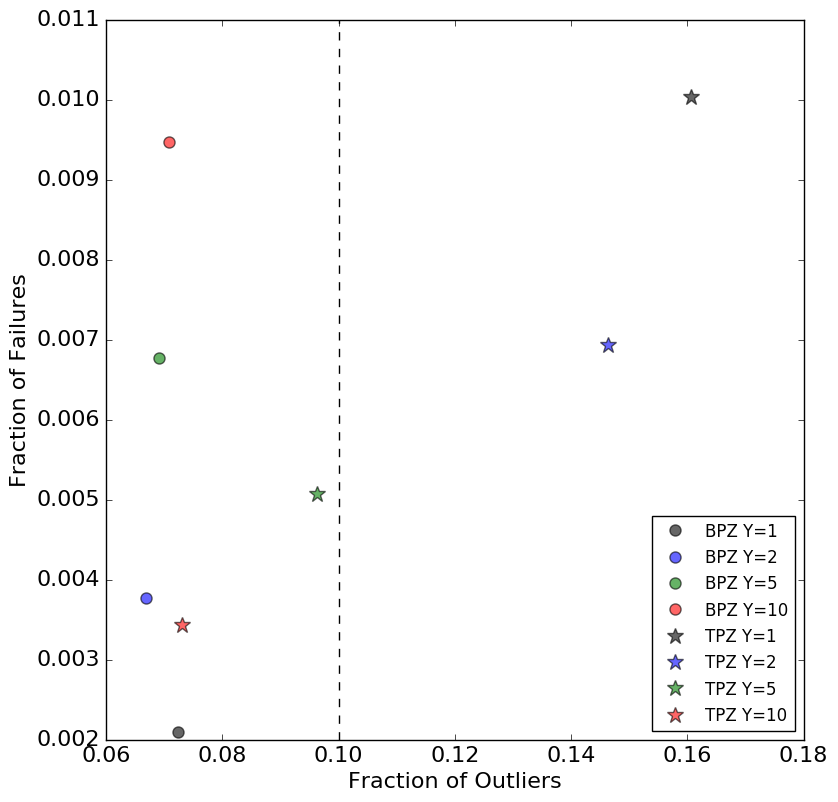
\includegraphics[width=8cm]{figures/stat_stat_fout_ffail.png}
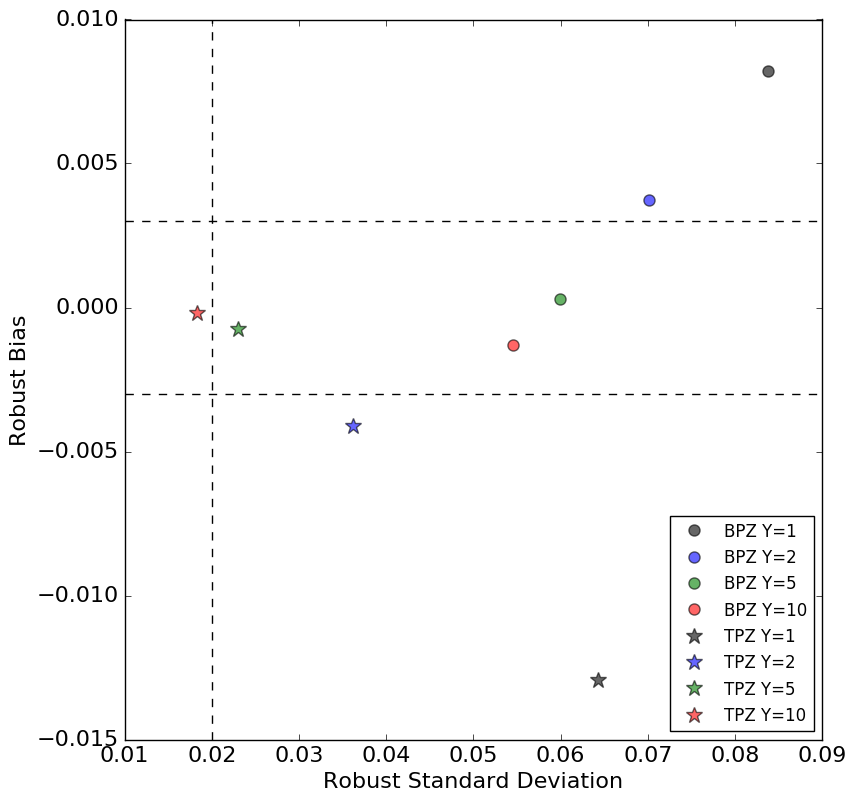
\includegraphics[width=8cm]{figures/stat_stat_std_bias.png}
\caption{Examples of how to compare statistical measures over $0.3 \leq z_\mathrm{phot} \leq 3.0$ from different photo-$z$ estimators by plotting one against the other: fraction of failures and outliers (left), and the robust bias and standard deviation (right). In this case we're comparing the statistical measures for TPZ and BPZ from photometry simulated for the LSST at years 1, 2, 5, and 10 (legend).  \label{fig:stat_stat}}
\end{center}
\end{figure*}

\begin{figure*}
\begin{center}
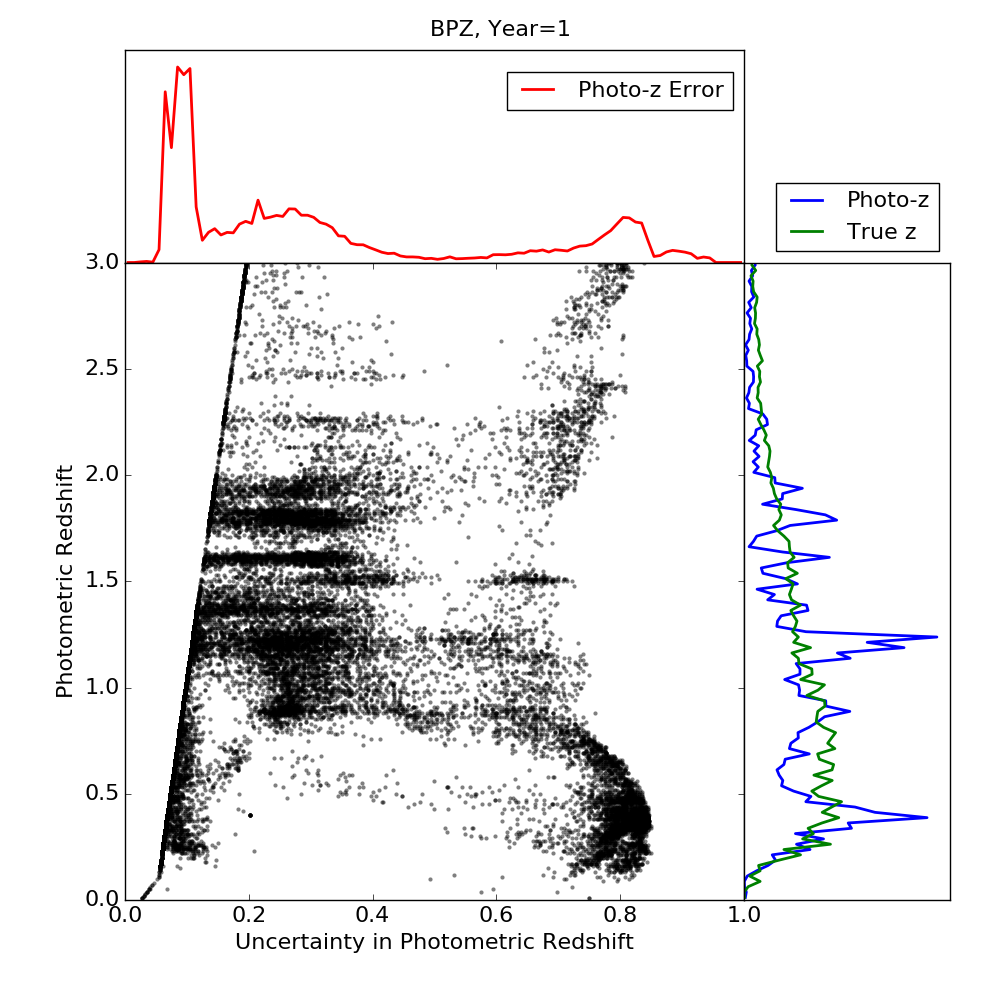
\includegraphics[width=6cm,trim={1cm 1cm 1cm 0cm}, clip]{figures/zp_zpe_bpz_euclid_1_2.png}
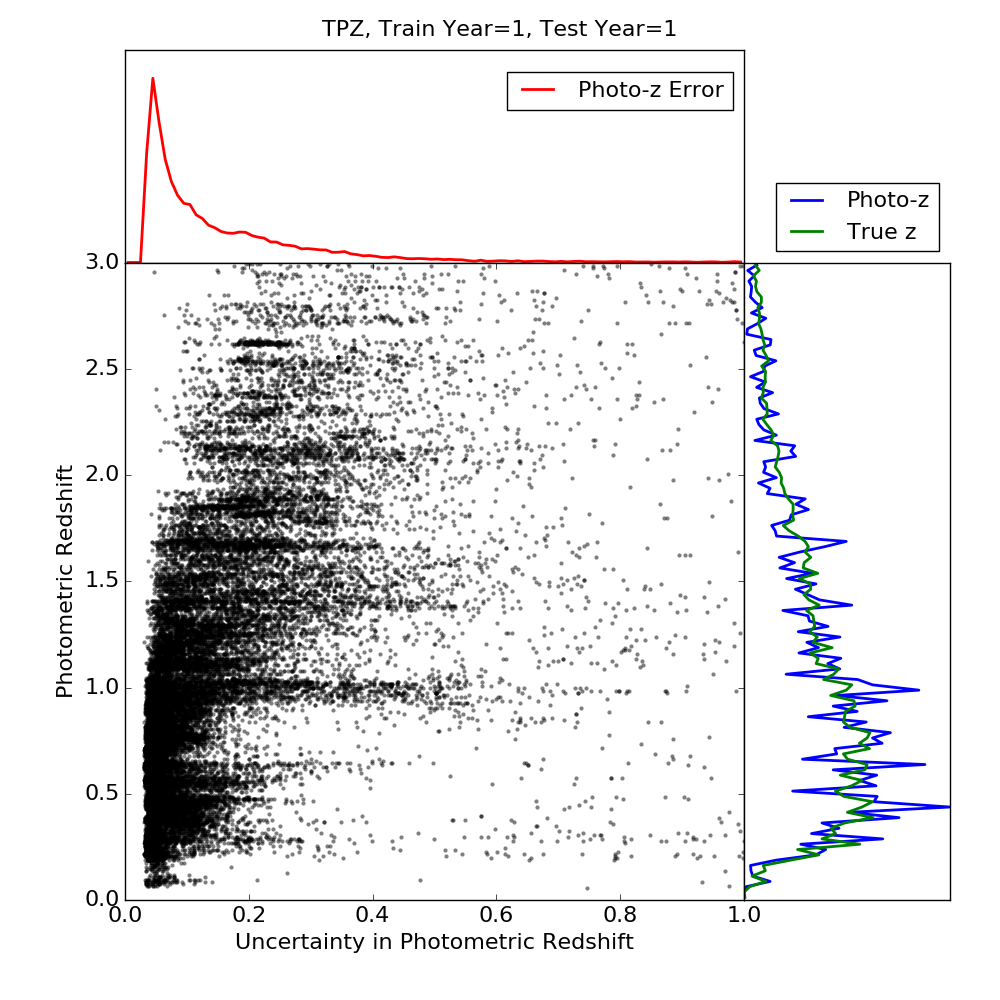
\includegraphics[width=6cm,trim={1cm 1cm 1cm 0cm}, clip]{figures/zp_zpe_tpz_euclid_1_1_2.png}
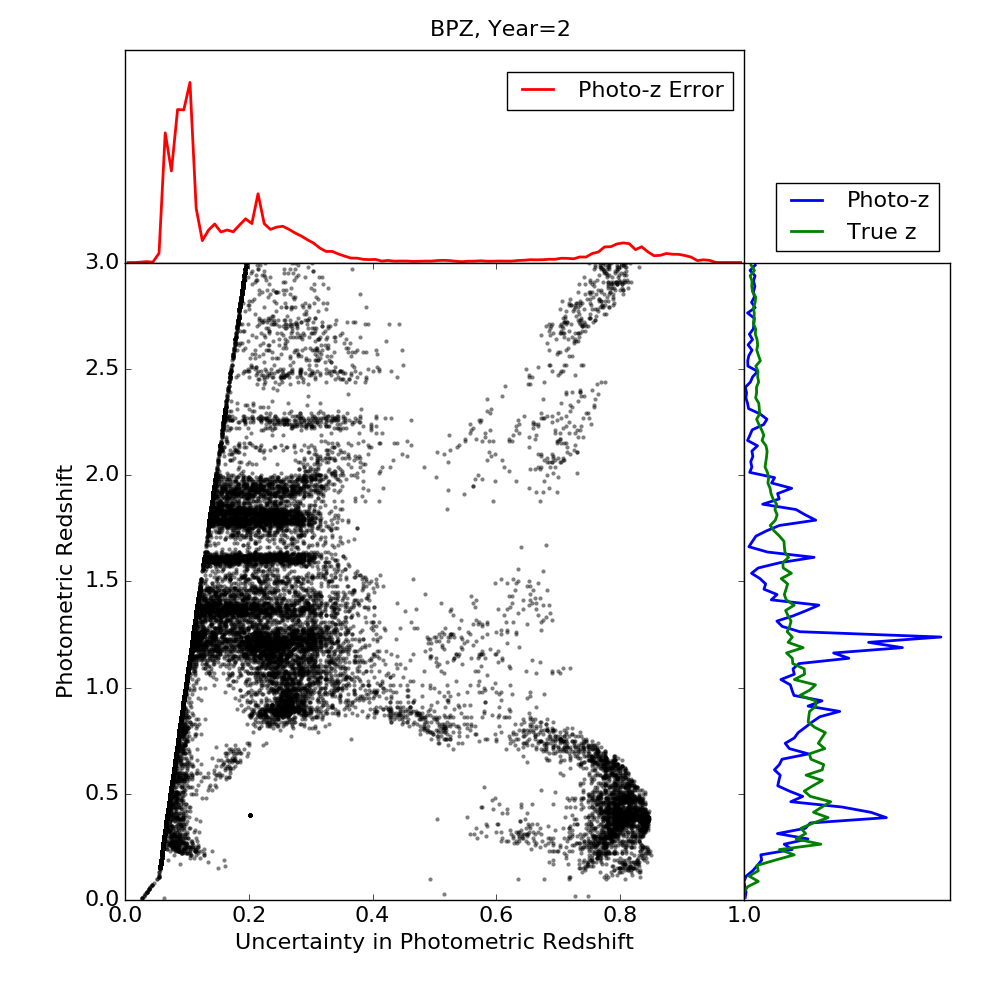
\includegraphics[width=6cm,trim={1cm 1cm 1cm 0cm}, clip]{figures/zp_zpe_bpz_euclid_2_2.png}
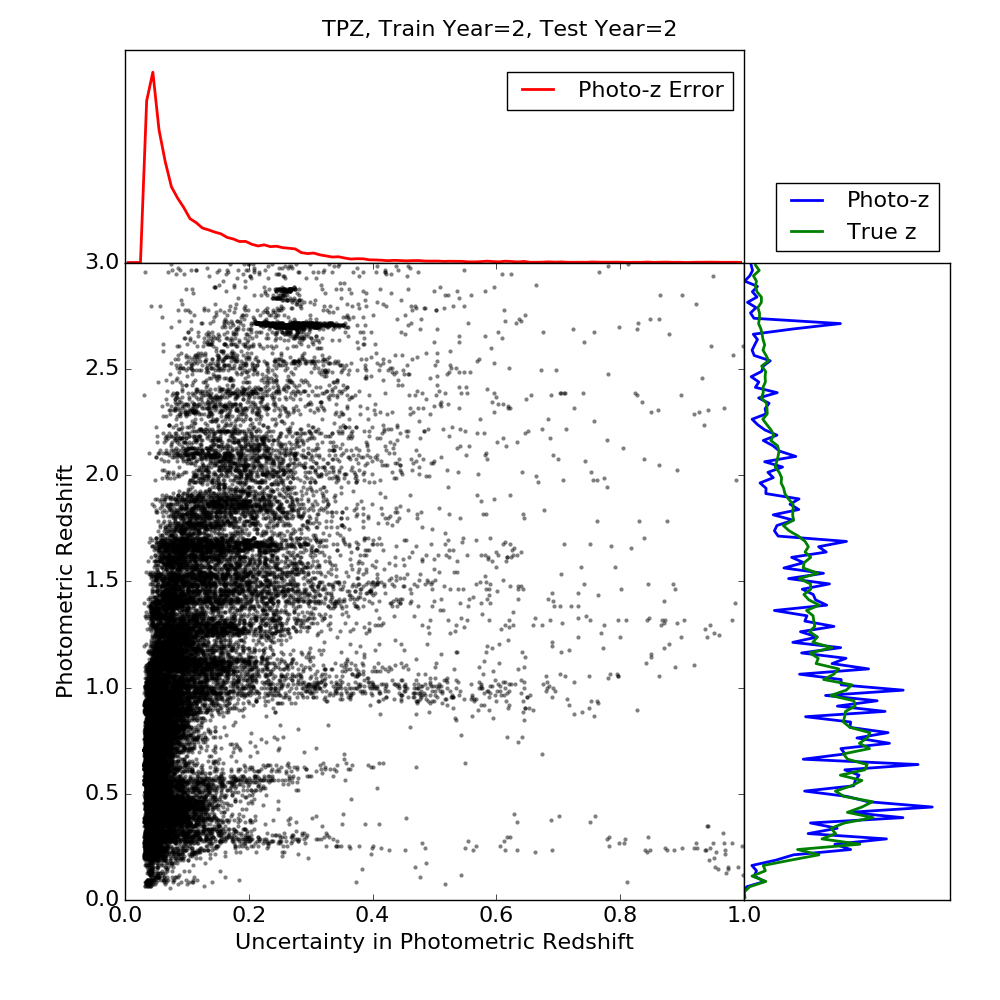
\includegraphics[width=6cm,trim={1cm 1cm 1cm 0cm}, clip]{figures/zp_zpe_tpz_euclid_2_2_2.png}
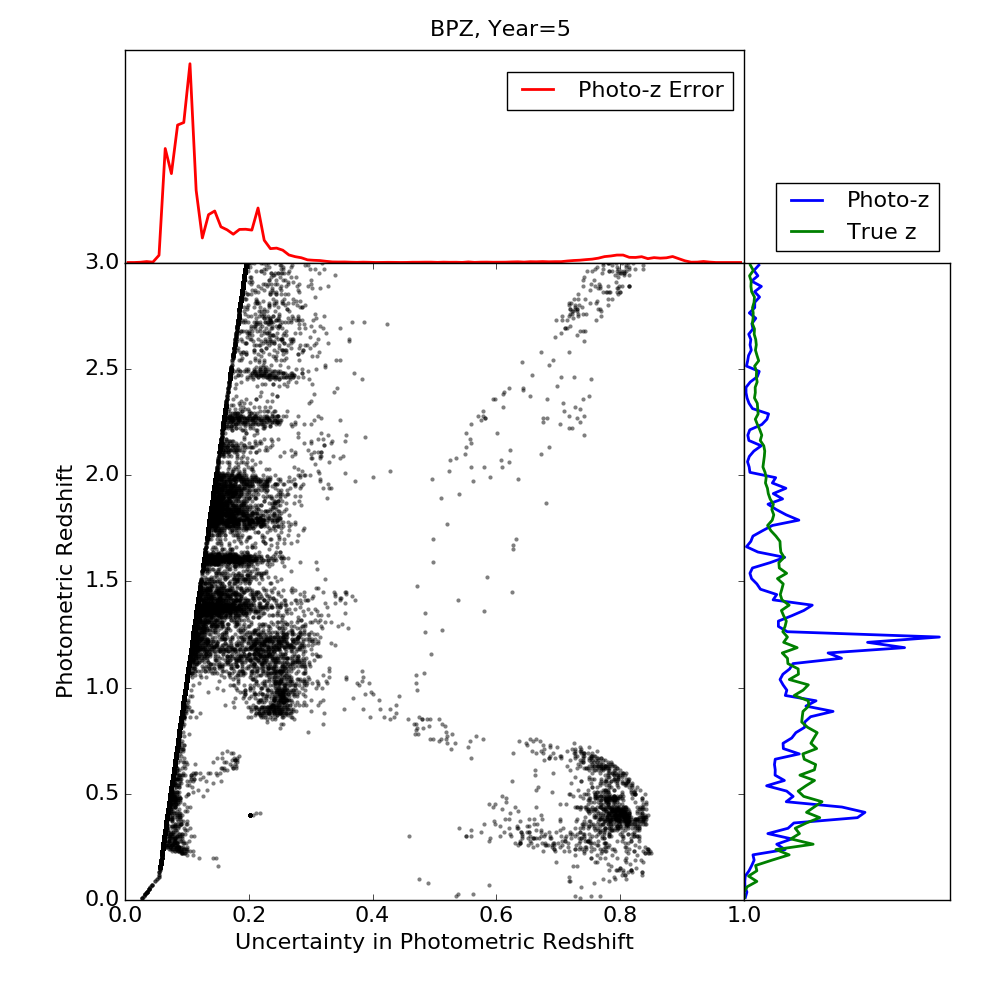
\includegraphics[width=6cm,trim={1cm 1cm 1cm 0cm}, clip]{figures/zp_zpe_bpz_euclid_5_2.png}
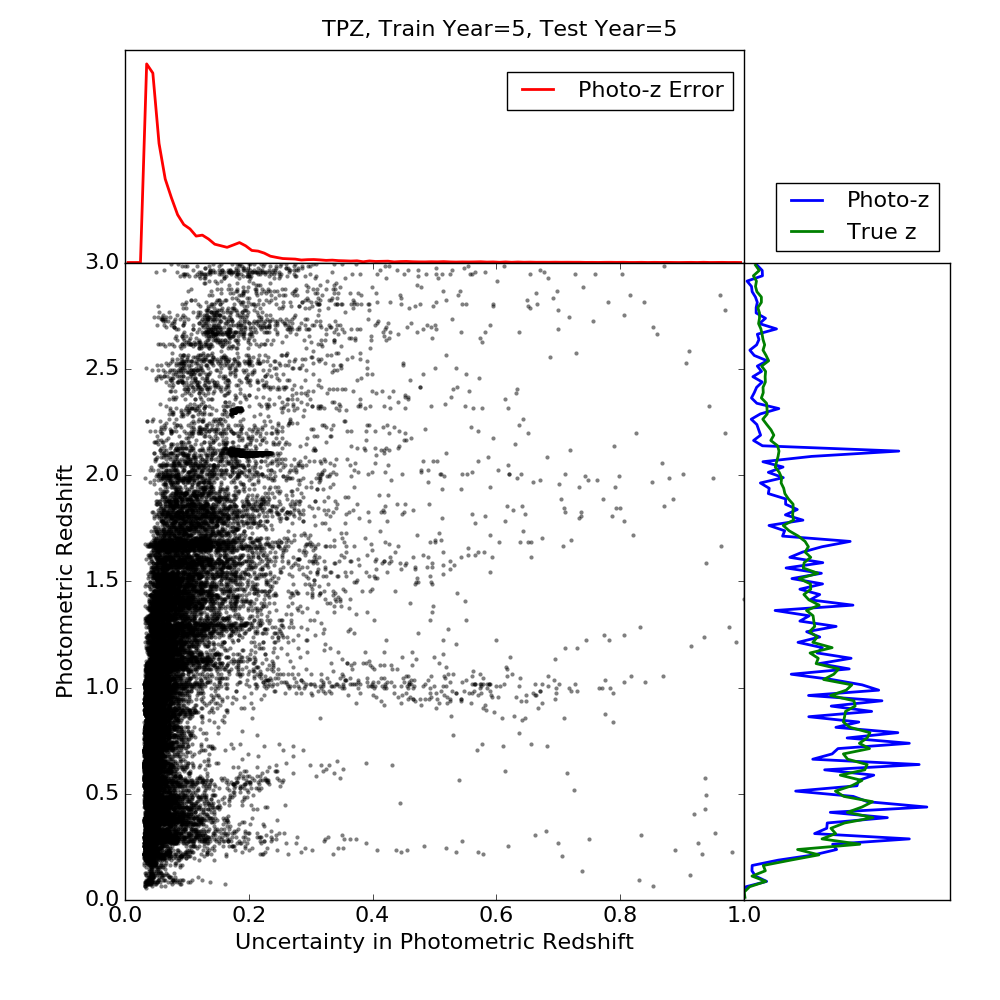
\includegraphics[width=6cm,trim={1cm 1cm 1cm 0cm}, clip]{figures/zp_zpe_tpz_euclid_5_5_2.png}
\caption{Examples of plot to compare the photo-$z$ uncertainty ($\delta z_\mathrm{phot}$) between algorithms with $z_\mathrm{phot}$--$\delta z_\mathrm{phot}$ plots from the BPZ (left) and TPZ (right) estimators for simulated catalogs with photometric uncertainties at 1, 2, and 5 years of LSST (top to bottom). Red lines show the distribution of photo-$z$ errors; blue and green lines compare the distributions of true and photometric redshifts. \label{fig:pzpze}}
\end{center}
\end{figure*}

\begin{figure*}
\begin{center}
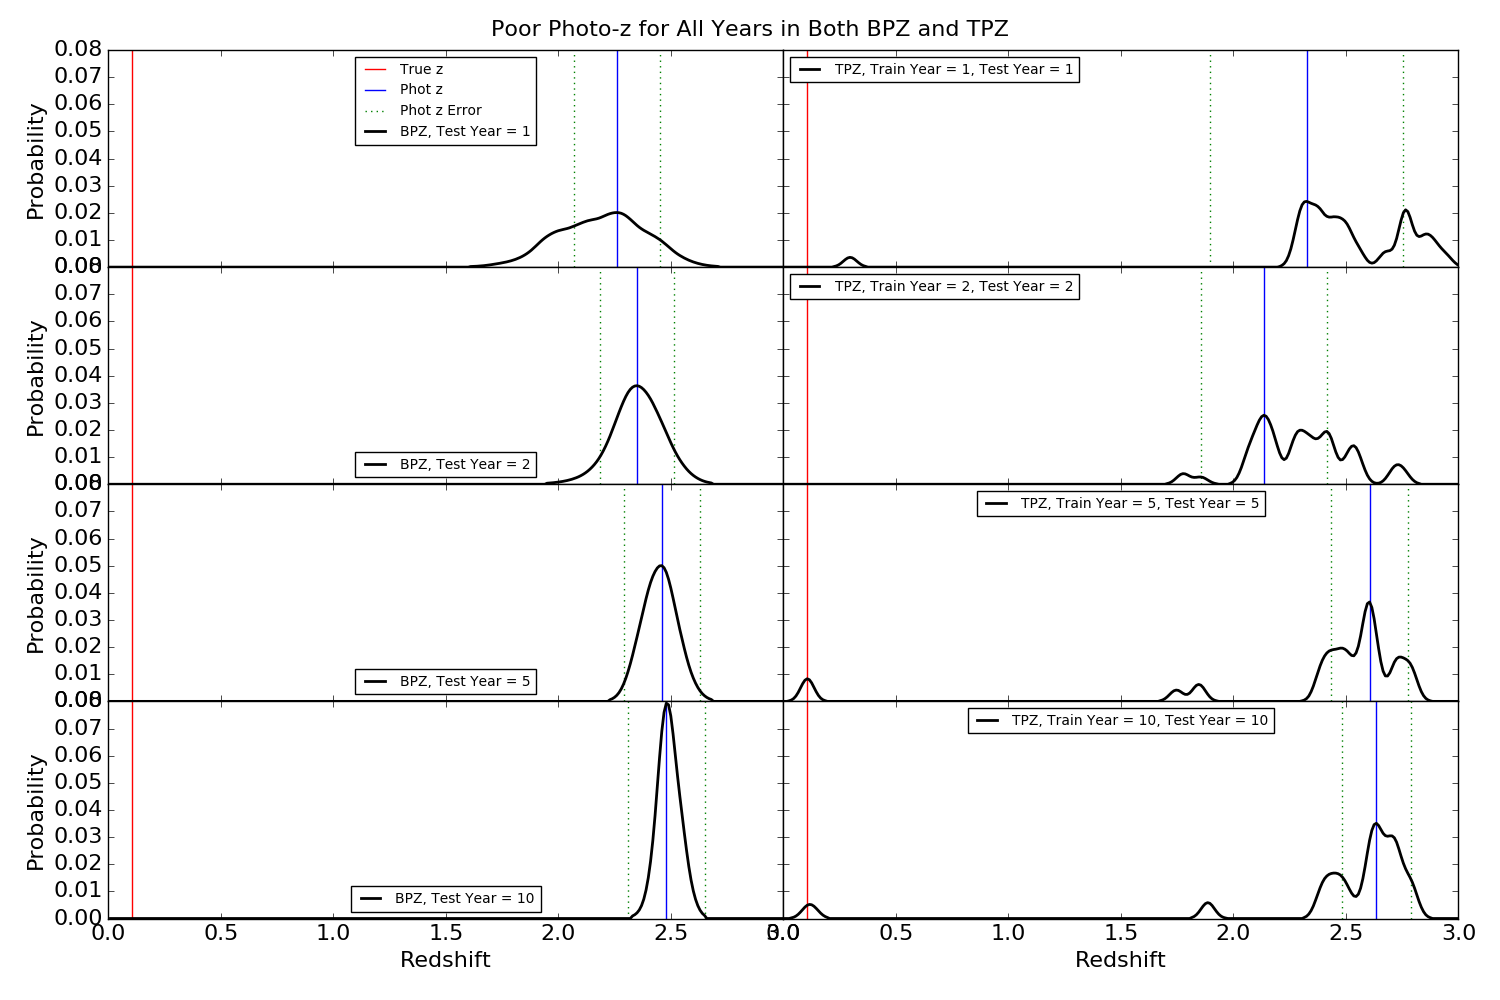
\includegraphics[width=13cm]{figures/zpdf_g4.png}
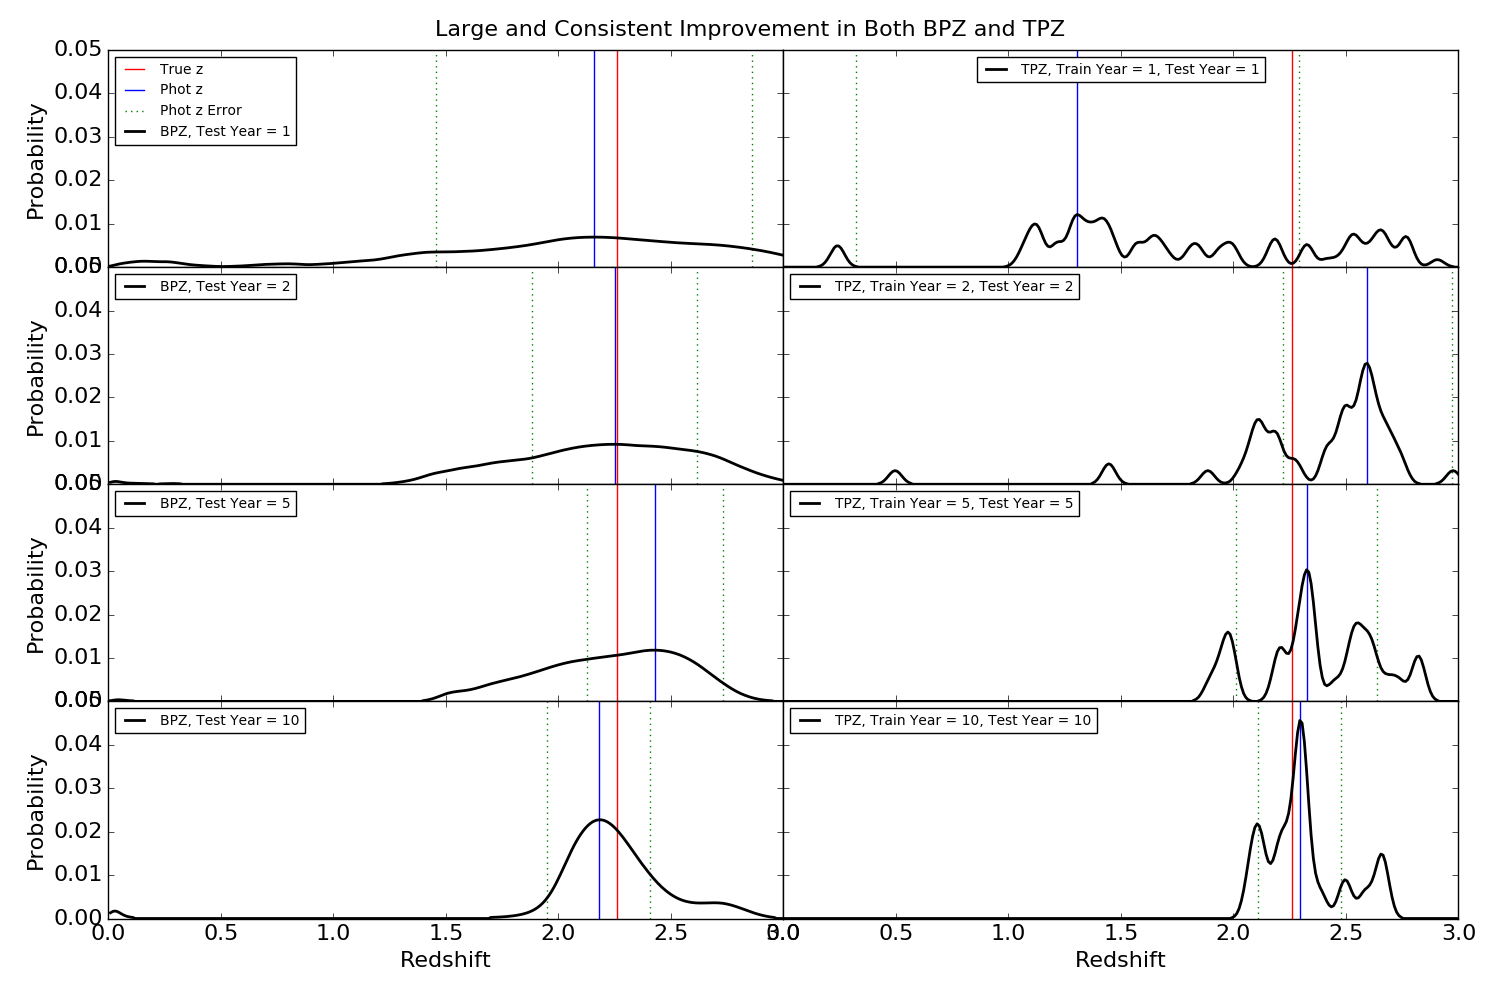
\includegraphics[width=13cm]{figures/zpdf_g7.png}
\caption{Examples of the posterior probability density functions for two test galaxies in all of our simulations: BPZ (left) and TPZ (right) for photometric uncertainties like 1, 2, 5, and 10 years of LSST (rows from top to bottom). In the top panel we choose a galaxy that return inaccurate and imprecise photo-$z$ from all 8 trials, and in the bottom panel we choose a galaxy that experienced a large and consistent improvement in photo-$z$ accuracy and precision from 1 to 10 years with both estimators.  \label{fig:zpdf}}
\end{center}
\end{figure*}

\begin{figure*}
\begin{center}
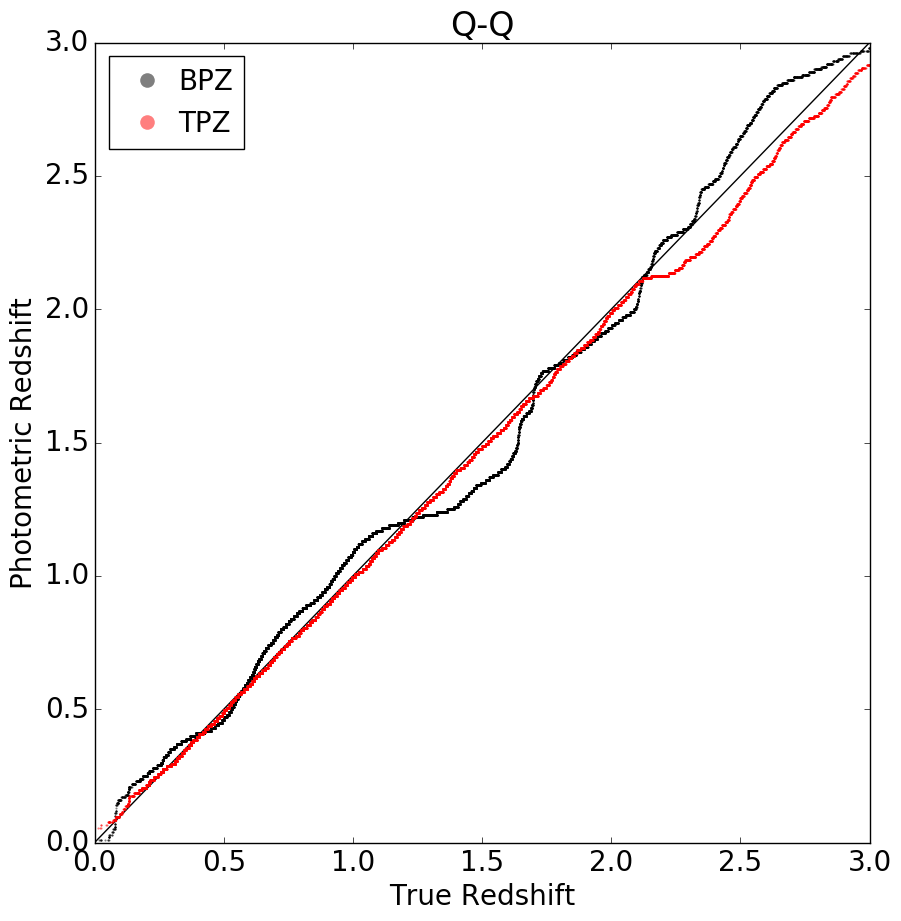
\includegraphics[width=10cm]{figures/qq_BPZ_TPZ.png}
\caption{Example of a Q-Q plot, using $z_\mathrm{true}$ and $z_\mathrm{phot}$, from the BPZ and TPZ estimators.}\label{fig:qq}
\end{center}
\end{figure*}